\chapter{Fachkonzeptschicht}
blabla
\colorbox{red}{BILD nur zum Testennnnnnn}
\begin{figure}
\centering
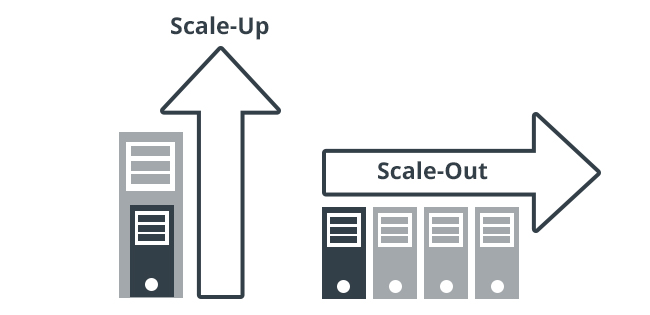
\includegraphics[width=0.7\textwidth]{resources/scales}
\caption[TEST]{TEST\protect\footnotemark}
\label{img:scales}
\end{figure}
\footnotetext{TEST: \url{https://magazin.kapilendo.de/den-supergau-verhindern-so-bereiten-sie-ihre-website-auf-einen-besucheransturm-vor/}, zugegriffen am 15. Januar 2017}
\section{Allgemein}

\begin{listingsboxJava}[label={lst:X}]{myJava}{Skript zur Initialisierung der Replikationsgruppe}
bla
\end{listingsboxJava}